\chapter{Homework 6 Solutions}
\begin{problem}[WebAssign, HW 6, 1]
Find the volume of the solid obtained by rotating the region bounded by
the given curves about the x-axis.
\[
 y=2-2x^2,\quad y=0.
\]
\end{problem}
\begin{proof}[Solution]
A good way to start the problem is to sketch the curve $y=2-x^2$ and the
area under the curve as as you can see in Figure \ref{fig:hw-6-1}.
\begin{figure}[htbp]
\centering
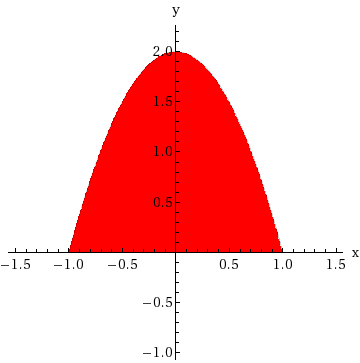
\includegraphics[scale=0.5]{hw-6-1}
\caption{Sketch of the area under the curve of $y=2-2x^2$.}
\label{fig:hw-6-1}
\end{figure}
Now, we are rotating about the $x$-axis so we want to find an expression
for the cross-sectional area, which depends on $y$, in terms of $x$
(remember, when we are rotating about an line or axis, our area $A$ will
depend on the variable perpendicular to our line or axis of rotation, in
this case $y$) in terms of our the variable we are varying over, i.e.,
$x$. Hence,
\[
  A(y)=\pi y^2=\pi\left(2-2x^2\right)^2.
\]
Hence, the volume of our solid, rotating about the $x$-axis will be given
by the integral
\begin{align*}
V=\int_{-1}^1 A(x)\diff x
&=\int_{-1}^1 \pi\left(2-2x^2\right)^2\diff x\\
&=\pi\int_{-1}^1 4-8x^2+4x^4\diff x\\
&=\pi\left(\left.4x-\frac{8}{3}x^3+\frac{4}{5}x^5\right|_{-1}^1\right),\\
\shortintertext{but since our graph is symmetric about the $y$-axis, we
  only need to integrate from $0$ to $1$ and then double the value}
&=2\pi\left(\left.4x-\frac{8}{3}x^3+\frac{4}{5}x^5\right|_{-1}^1\right)\\
&=2\pi\left(4-\frac{8}{3}+\frac{4}{5}-\left(4\cdot 0-\frac{8}{3}\cdot
  0^3-\frac{4}{5}\cdot 0^5\right)\right)\\
&=2\pi\left(4-\frac{8}{3}+\frac{4}{5}\right)\\
&=2\pi\left(\frac{4\cdot 3\cdot 5-8\cdot 5+4\cdot 3}{3\cdot 5}\right)\\
&=2\pi\left(\frac{60-40+12}{15}\right)\\
&=\frac{64\pi}{15}
\end{align*}
\end{proof}


\begin{problem}[WebAssign, HW 6, 2]
  Find the volume $V$ of the solid obtained by rotating the region bounded by
  the given curves about the specified line.
  \[
    y=2\sqrt{49-x^2},\quad y=0,\quad x=4,\quad x=5;\text{ about the $x$-axis.}
  \]
\end{problem}
\begin{proof}[Solution]
We begin by sketching the region like so
[htbp]
\begin{figure}[htbp]
  \centering
 \includegraphics{mhw-6-2}
  \caption{Volume of solid obtain by rotating the region bounded by
    $y=2\sqrt{49-x^2}$, $y=0$, $x=4$, and $x=5$.}
  \label{fig:hw-6-2}
\end{figure}
\end{proof}


\begin{problem}[WebAssign, HW 6, 3]
\end{problem}
\begin{proof}[Solution]
\end{proof}


\begin{problem}[WebAssign, HW 6, 4]
\end{problem}
\begin{proof}[Solution]
\end{proof}


\begin{problem}[WebAssign, HW 6, 5]
\end{problem}
\begin{proof}[Solution]
\end{proof}


\begin{problem}[WebAssign, HW 6, 6]
\end{problem}
\begin{proof}[Solution]
\end{proof}


\begin{problem}[WebAssign, HW 6, 7]
\end{problem}
\begin{proof}[Solution]
\end{proof}


\begin{problem}[WebAssign, HW 6, 8]
\end{problem}
\begin{proof}[Solution]
\end{proof}

%%% Local Variables:
%%% mode: latex
%%% TeX-master: "../MA166-HW-Current"
%%% End:
